\documentclass[../main.tex]{subfiles}

\begin{document}
%%%%%%%%%%%%%
%           %
% WX MAXIMA %
%           %
%%%%%%%%%%%%%

\chapter{WX MAXIMA Cheatsheet}
Mehrzeilige Eingabe mit Enter. Shift-Enter um auszurechnen.

\section{Grundlagen}
\begin{tabularx}{1.0\textwidth} { 
    >{\centering\arraybackslash}X 
    >{\centering\arraybackslash}X  }
    a+b,a-b,a*b,a/b & Addition, Subtraktion, Multiplikation, Division
    \\ [7pt]
    \hline
    a**b & Potenzierung
    \\ [7pt]
    \hline
    sqrt(x),exp(x),log(x) & Wurzel, Exponentialfunktion, natürlicher Logarithmus
    \\ [7pt]
    \hline
    sin(x),cos(x),tan(x) & Winkelfunktionen
    \\ [7pt]
    \hline
    asin(x),acos(x),atan(x) & Arkusfunktionen
    \\ [7pt]
    \hline
    float(x) & Umwandlung aller Zahlen im Ausdruck x in Gleitkommazahlen
    \\ [7pt]
    \hline
    floor(x),round(x) & Abschneiden und Runden
    \\ [7pt]
    \hline
    \%pi,\%e,\%i & Pi, Eulersche Zahl und imaginäre Einheit
    \\ [20pt]
\end{tabularx}
Alle Zahlen müssen explizit multipliziert werden, um also "2x" zu schreiben muss man "2*x" eingeben.

\subsection{Einfache Operationen}
\begin{tabularx}{1.0\textwidth} { 
    >{\centering\arraybackslash}X 
    >{\centering\arraybackslash}X  }
    a:b & Zuweisung; der Wert von b wird dem Symbol a zugewiesen.
    \\ [7pt]
    \hline
    kill(a) & a löschen 
    \\ [7pt]
    \hline
    values & Liste aller mit einem Wert belegten Benutzervariablen
    \\ [7pt]
    \hline
    kill(x1,x2,. . .) & Löschen der Variablen x1, x2, . . .
    \\ [7pt]
    \hline
    ev(expr,opts) & Auswerten des Ausdrucks expr mit den optionalen Parametern opts
    \\ [7pt]
    \hline
    expr,opts & Verkürzte Form des Auswertebefehls. Optionen:var=val. . . Einsetzen eines Werteseval. . . nochmaliges Auswerteninfeval. . . wiederholtes Auswertennumer. . . Gleitkommadarstellung
    \\ [7pt]
    \hline
    xthru(expr) & Auf gleichen Nenner bringen
    \\ [7pt]
    \hline
    ratsimp(expr) & Vereinfachen und auf gleichen Nenner bringen
    \\ [7pt]
    \hline
    expand(expr) & Expandieren (Ausmultiplizieren)
    \\ [7pt]
    \hline
    map(expand,expr) & Zähler und Nenner getrennt expandieren
    \\ [7pt]
    \hline
    num(expr),denom(expr) & Zähler bzw. Nenner von expr
    \\ [7pt]
\end{tabularx}

\section{Systemvariablen}
\begin{tabularx}{1.0\textwidth} { 
    >{\centering\arraybackslash}X 
    >{\centering\arraybackslash}X  }
    fpprintprec & Anzahl der signifikanten Stellen bei der Ausgabe vonGleitkommazahlen
    \\ [7pt]
    \hline
    float & Umwandlung aller Zahlen in Gleitkommazahlen(Default:false)
    \\ [7pt]
    \hline
    numer & Wiefloat, veranlasst zusätzlich mathematischeFunktionen zur Auswertung in Gleitkommadarstellung(Default:false)
    \\ [7pt]
\end{tabularx}

\section{Logische Ausdrücke}
\begin{tabularx}{1.0\textwidth} { 
    >{\centering\arraybackslash}X 
    >{\centering\arraybackslash}X  }
    true,false & Logische Konstantenwahrundfalsch
    \\ [7pt]
    \hline
    =,\#,<,<=,>,>= & Vergleichsoperatorengleich, ungleich, kleiner, kleinergleich, größer, größer gleich
    \\ [7pt]
    \hline
    and,or,not & Logische Operatoren und, oder, nicht
    \\ [7pt]
    \hline
    equal(a,b) & Überprüfung, ob die beiden Ausdrücke a und b denselben Wert ergeben
    \\ [7pt]
    \hline
    is(expr) & Auswerten des Vergleichsausdrucks expr zu true, false oder unknown
    \\ [7pt]
    \hline
\end{tabularx}

\section{Summen und Grenzwerte}
\begin{tabularx}{1.0\textwidth} { 
    >{\centering\arraybackslash}X 
    >{\centering\arraybackslash}X  }
    inf,minf & Symbole für unendlich und negativ unendlich
    \\ [7pt]
    \hline
    sum(expr,i,i0,i1) & Summe $\sum\limits_{i=i0}^{i1}expr$
    \\ [7pt]
    \hline
    limit(expr,i,i0) & Grenzwert $\lim\limits_{i\to i0}expr$
    \\ [7pt]
    \hline
    simpsum & Systemvariable, veranlasst die Berechnung von Summen mit symbolischen Indexgrenzen (zB inf) (Default:false)
    \\ [7pt]
    \hline
    Beispiel & sum(1/n**2,n,1,inf),simpsum=true;
    \\ [7pt]
    \hline
\end{tabularx}


\section{Differenzieren und Integrieren}
\begin{tabularx}{1.0\textwidth} { 
    >{\centering\arraybackslash}X 
    >{\centering\arraybackslash}X  }
    diff(expr,x[,n]) & n-te Ableitung des Ausdrucks expr nach der Variablen x; die Angabe von n ist optional, Default: 1.
    \\ [7pt]
    \hline
    integrate(expr,x) & Unbestimmtes Integral des Ausdrucks expr mit der Integrationsvariablen x
    \\ [7pt]
    \hline
    integrate(expr,x,x0,x1) & Bestimmtes Integral des Ausdrucks expr mit der Integrationsvariablen x zwischen den Grenzen x0 und x1
    \\ [20pt]
\end{tabularx}
Für partielle int/diff: diff(f(x,y),x)

\section{Gleichungen}
\begin{tabularx}{1.0\textwidth} { 
    >{\centering\arraybackslash}X 
    >{\centering\arraybackslash}X  }
    solve(eqn,var) & Lösen der algebraischen Gleichung eqn nach der Variablen var
    \\ [7pt]
    \hline
    solve(eqns,vars) & Lösen einer Liste eqns von algebraischen Gleichungen nach den Variablen in der Liste vars
    \\ [7pt]
    \hline
    allroots(p) & Numerische Berechnung aller Nullstellen des Polynoms p
    \\ [7pt]
    \hline
    find\_root(expr,x1,x2) & Numerische Ermittlung einer Nullstelle des Ausdrucks expr innerhalb des Intervalls x1...x2
    \\ [7pt]
    \hline
\end{tabularx}

\subsection{Beispiele}
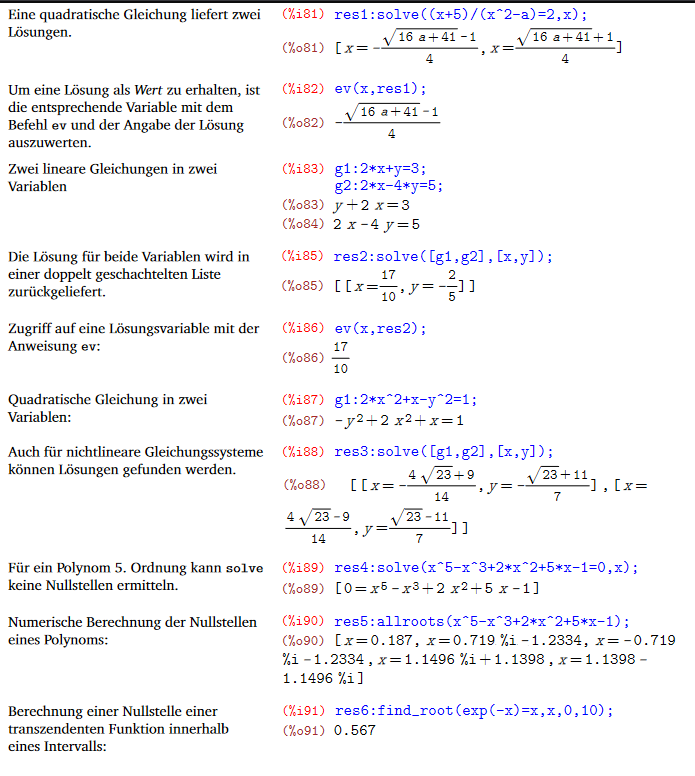
\includegraphics[width=100mm,scale=1]{wx_maxima_examples}

\section{Funktionen}
f(x1,x2,. . .):=expr

\iffalse
\begin{tabularx}{1.0\textwidth} { 
    >{\centering\arraybackslash}X 
    >{\centering\arraybackslash}X  }
    &
    \\ [7pt]
    \hline
    &
    \\ [7pt]
    \hline
    &
    \\ [7pt]
    \hline
    &
    \\ [7pt]
    \hline
    &
    \\ [7pt]
    \hline
\end{tabularx}
\fi

\end{document}